\section{Experimental Results}  \label{sec:exp}

\subsection{Experimental Setup}
We did experiment on one indoor dataset, the Berkeley Dataset, and one outdoor dataset, the NTU Traffic dataset.
We also exploit two missing patterns: random missing and consecutive missing.
\subsubsection{Datasets}

\paragraph*{Berkeley Dataset}

The Intel Berkeley Research lab dataset~\cite{berkeley2004lab} records temperature, humidity, light, and voltage for 54 sensors (with one sensor completely missing) for which locations are given (see Figure \ref{berkeley_lab}) during February 28th and April 5th, 2004 in an indoor lab environment.
The dataset includes 2.3M sensor observations, over 210K samples along the temporal dimension.
Since the completeness of data degrades after 10000 samples, in our experiments only the first 2500, 5000, or 10000 samples were used.
We found the performances of models are similar in these three cases, therefore we report only results from 5000 samples. 

\begin{figure}[H]
\centering
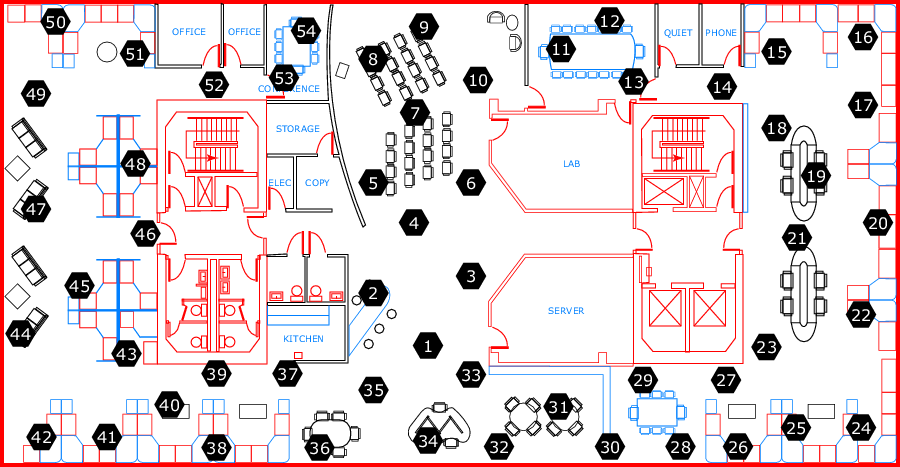
\includegraphics[scale=0.25]{berkeley_lab.png}
\caption{Intel Berkeley Research Lab Floorplan} \label{berkeley_lab}
\end{figure}

\paragraph*{NTU Traffic Dataset}

The NTU Traffic Dataset records the temperature, humidity, and voltage conditions of 20 sensor nodes and one gateway node.
This dataset, collected by the Bio-industrial Department at National Taiwan University, was recorded over a 2.5 year time period ending in 2011 in an outdoor location high traffic area in Taipei, Taiwan\cite{liu2011developed}.
The sampling rate is roughly once every 30 minutes.
Along the temporal dimension, we use the entire range which consists of roughly 43K time stamps.
%This dataset only reveals 8 

Note that for both Berkeley and NTU datasets, simple preprocessing rules were applied to remove apparent outliers.
In the Berkeley dataset, observations are removed if temperature \mbox{$>100\degc$}, temperature \mbox{$<5\degc$}, or humidity \mbox{$<16\%$}.
In the traffic dataset, observations are removed if temperature \mbox{$>100\degc$}, temperature \mbox{$<5\degc$}, or humidity \mbox{$<16\%$}.
\begin{figure}[H]
\centering
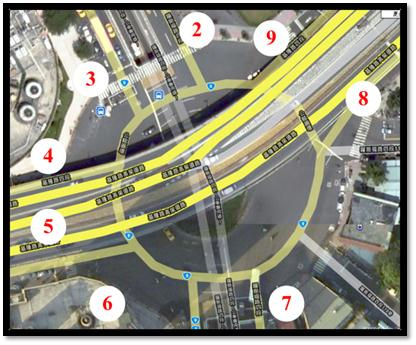
\includegraphics[scale=0.5]{traffic_wsn.png}
\caption{NTU Traffic Sensor Deployment Configuration (8 sensors of 20 shown)}
\end{figure}

%\subsubsection{Dataset Preparation}

%\paragraph{Berkeley Dataset Outlier Removal and Gridding}

%Gridding : Dataset falls on even 30s intervals for the first 5000 time steps (which is all we consider), so no additional gridding need be performed.
%Outlier Filtering : We use some simple rules to removed apparent errors. Observation removed if temperature \mbox{$>100\degc$}, temperature \mbox{$<5\degc$}, or humidity \mbox{$<16\%$}.

%\paragraph*{Traffic Dataset Outlier Removal and Gridding}


%Gridding : The original dataset recorded most readings at around the $xx:03$ and $xx:33$ minute marks, so a $6$ min window centered at these points captured the data for $30$ minute internal readings. Where more than one reading was recorded for a given node within a given window, the closest to the $3$ or $33$ minute mark was chosen. The full length of the dataset was used, which consists of $\approx 43$K 

%Outlier Filtering : Observation removed if temperature \mbox{$<5\degc$} or \mbox{$>60\degc$} or if humidity \mbox{$<10\%$} or \mbox{$>100\%$}.
\subsubsection{Missing Data Generation}

%Datasets of various lengths are produced from the single input dataset for our experiments, namely 2500, 5000, and 10000.
%There is an initially missing portion of the observations which can be considered Missing At Random (MAR).To this, we impose two different types of Missing Completely At Random (MCAR) sampling techniques to build validation and testing datasets.

Although both datasets intrinsically have missing readlings, we cannot use those for evaluation because their true values are unknown.
Instead we devised two strategies to produce artificial missing data.
\paragraph*{Random Missing Pattern}

This pattern reflects choosing a random time and random sensor to be missing and hence removed from the training set.
Here we follow the standard evaluation process in machine learning to divide the data into training, validation, and testing sets.

We define two variables $x$ and $y$ during our experiment, and the X-axis of the resulting plot varies with $x$.

\begin{itemize}
\item $10\%$ of the existing readings are randomly selected (without replacement) to be the validation set
\item $y\%$ of the existing readings are randomly selected (without replacement) to be the testing set
\item The remaining readings (x\%) are part of the training set. That is, x+y+10=100 that accounts for all the observed readings.
\end{itemize}
\paragraph*{Consecutive Missing Pattern}

This pattern reflects testing the effect of all data missing after a certain point in time.
We define two values $x$ and $y$ as follows.

\begin{itemize}
\item Here, we have the last $y\%$ of time covered as missing, and the prior $10\%$ to that is considered as the validation data.
\item The sensor node numbers ``covered up'' in the validation and testing for the Berkeley and Traffic datasets are ${4,19,45}$ and ${2,4,6,8,10,14,17,19,20,21}$, respectively.
Note that node $21$ of the Traffic dataset is the gateway node.
\end{itemize}

We exploit the commonly used metric of root-mean-square-error (RMSE) to measure the difference between the predicted values and the ground truth.
